% !TEX root = ../main.tex

\newcommand{\englishQuote}[1]{“\textit{#1}”}

%----------------------------------------
%   SECTION TITLE
%----------------------------------------

\label{chap:questions}

%----------------------------------------
%   SECTION CONTENT
%----------------------------------------

\chapter{Guideline and Structure}
\section{Guidelines for the structure of study documentation: }

A study is always an independent and specific project. For this reason, there are no strict
and static guidelines for the structure of the study, but rather a number of conceptual
aspects and guidelines that must be taken into account. These must be reflected in the
presentation. However, it is crucial that the description of the study is consistent in itself.
Objectives, questions, prerequisites, methods, implementation and descriptive statistics
must be presented in a comprehensible, complete and understandable manner.
In the context of the course Introduction to Statistics and Biometry, this structure is to be
realized in four subtasks, and documented accordingly. The study topic should be chosen
individually by each group.
The overall task is to document the entire study. The description of the content should
not exceed 5-8 pages. Please note that this is important: This page limit refers only to
the documentation of the content. The actual questionnaire as well as the pure raw data
processing by means of descriptive statistics are not subject to any limitation with
regard to the number of pages, since they depend on the chosen topic as well as the
presentation of the key figures and distributions. The overall documentation will
therefore naturally contain more than the 5-8 pages.(Professor Dr. Christian Thies)

\pagebreak
\chapter{Draft}
\section{Framework}

The aim is to conduct a cross-sectional study to authentically capture the opinions of students regarding the \gls{dt} in the full solidarity model (instead of Naldo in the partial solidarity model). Our goal is to gain a comprehensive overview of approval, rejection, skepticism, or enthusiasm. This study will help us make an informed decision on whether and how the Deutschlandticket should influence our daily lives. By directly capturing the current mood of the student body, we aim to create a solid foundation for an informed decision.

\section{Research Question}

What is the level of acceptance among the students of Reutlingen University for a Deutschlandticket in the full solidarity model?

\section{Approach}
\subsection{Timeline}
% The agenda consisted of creating a prototype, testing that prototype with a representative group, implementing fixes, and launching.
After deciding on a platform to conduct our survey on we started by creating a prototype to identify possible issues that might arise. After testing that prototype on about 40 participants -- that reached the survey through our marketing material on the first day and were therefore representative of the actual participants -- we modified the order of some question groups and adjusted (increased) the range for numeric inputs based on feedback. The actual data collection began on the next day with participants reaching our survey through our physical marketing material as well as social media. The following days we gradually increased the amount of marketing material on the campus and \textit{re}uploaded the posts multiple times.

\subsection{Distribution / Marketing}

The survey was distributed to students via the STUPA email and the new university app "MyHSRT". Posters were placed across all campus buildings. Additionally, table-tents were set up in many buildings, with a focus on the library, cafeteria, and active classrooms. Table-tents are small, tent-shaped displays used for advertising or informational purposes, typically placed on tables in restaurants, events, or other venues.

We also used word of mouth, spreading information through chat groups of different study programs. To complement these efforts, we created a social media campaign for Instagram. This campaign consisted of multiple posts and was coordinated with the university marketing team to be shared via the official HSRT Instagram accounts.

\begin{multicols}{3}
    \begin{figure}[H]
       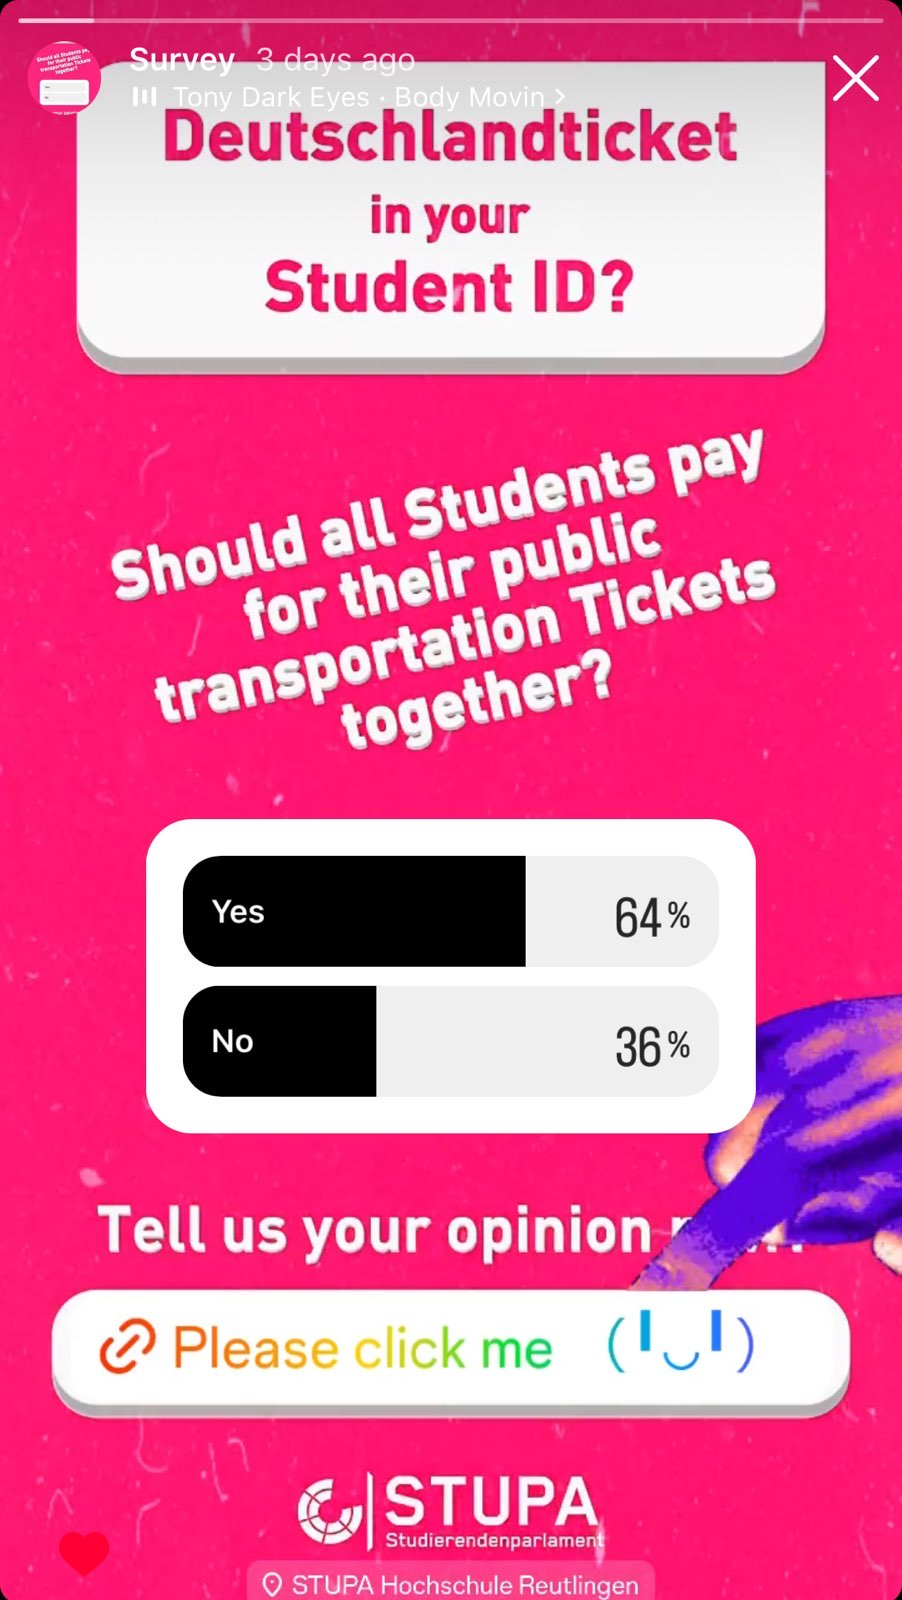
\includegraphics[width=0.8\textwidth]{Content/Images/Story.jpeg}
      \caption{Instagram Story 1}
       \label{fig:InstagramStory1}
    \end{figure}
    \columnbreak
    \begin{figure}[H]
       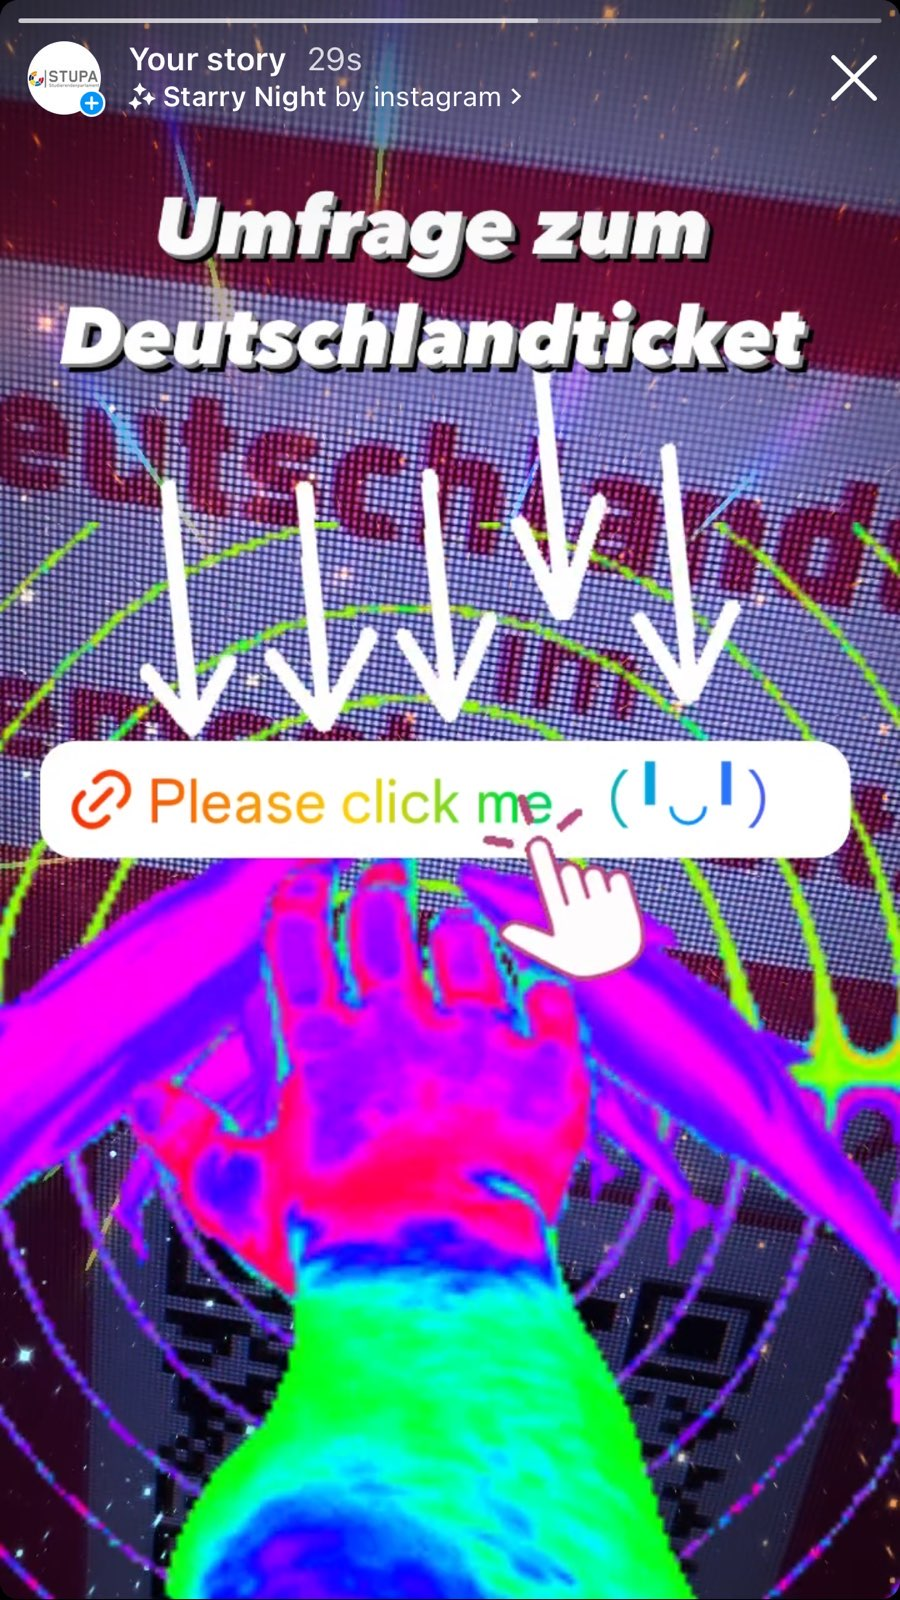
\includegraphics[width=0.8\textwidth]{Content/Images/Story_2.jpeg}
       \caption{Instagram Story 2}
       \label{fig:InstagramStory2}
    \end{figure}
    \columnbreak
    \begin{figure}[H]
        \vspace{0.3\textwidth}
        
\includegraphics[width=0.8\textwidth]{Content/Images/IG_Square.png}
        \caption{Instagram Post}
        \label{fig:InstagramPost}
    \end{figure}
\end{multicols}

\begin{multicols}{3}
    \begin{figure}[H]
        \vspace{0.3\textwidth}
        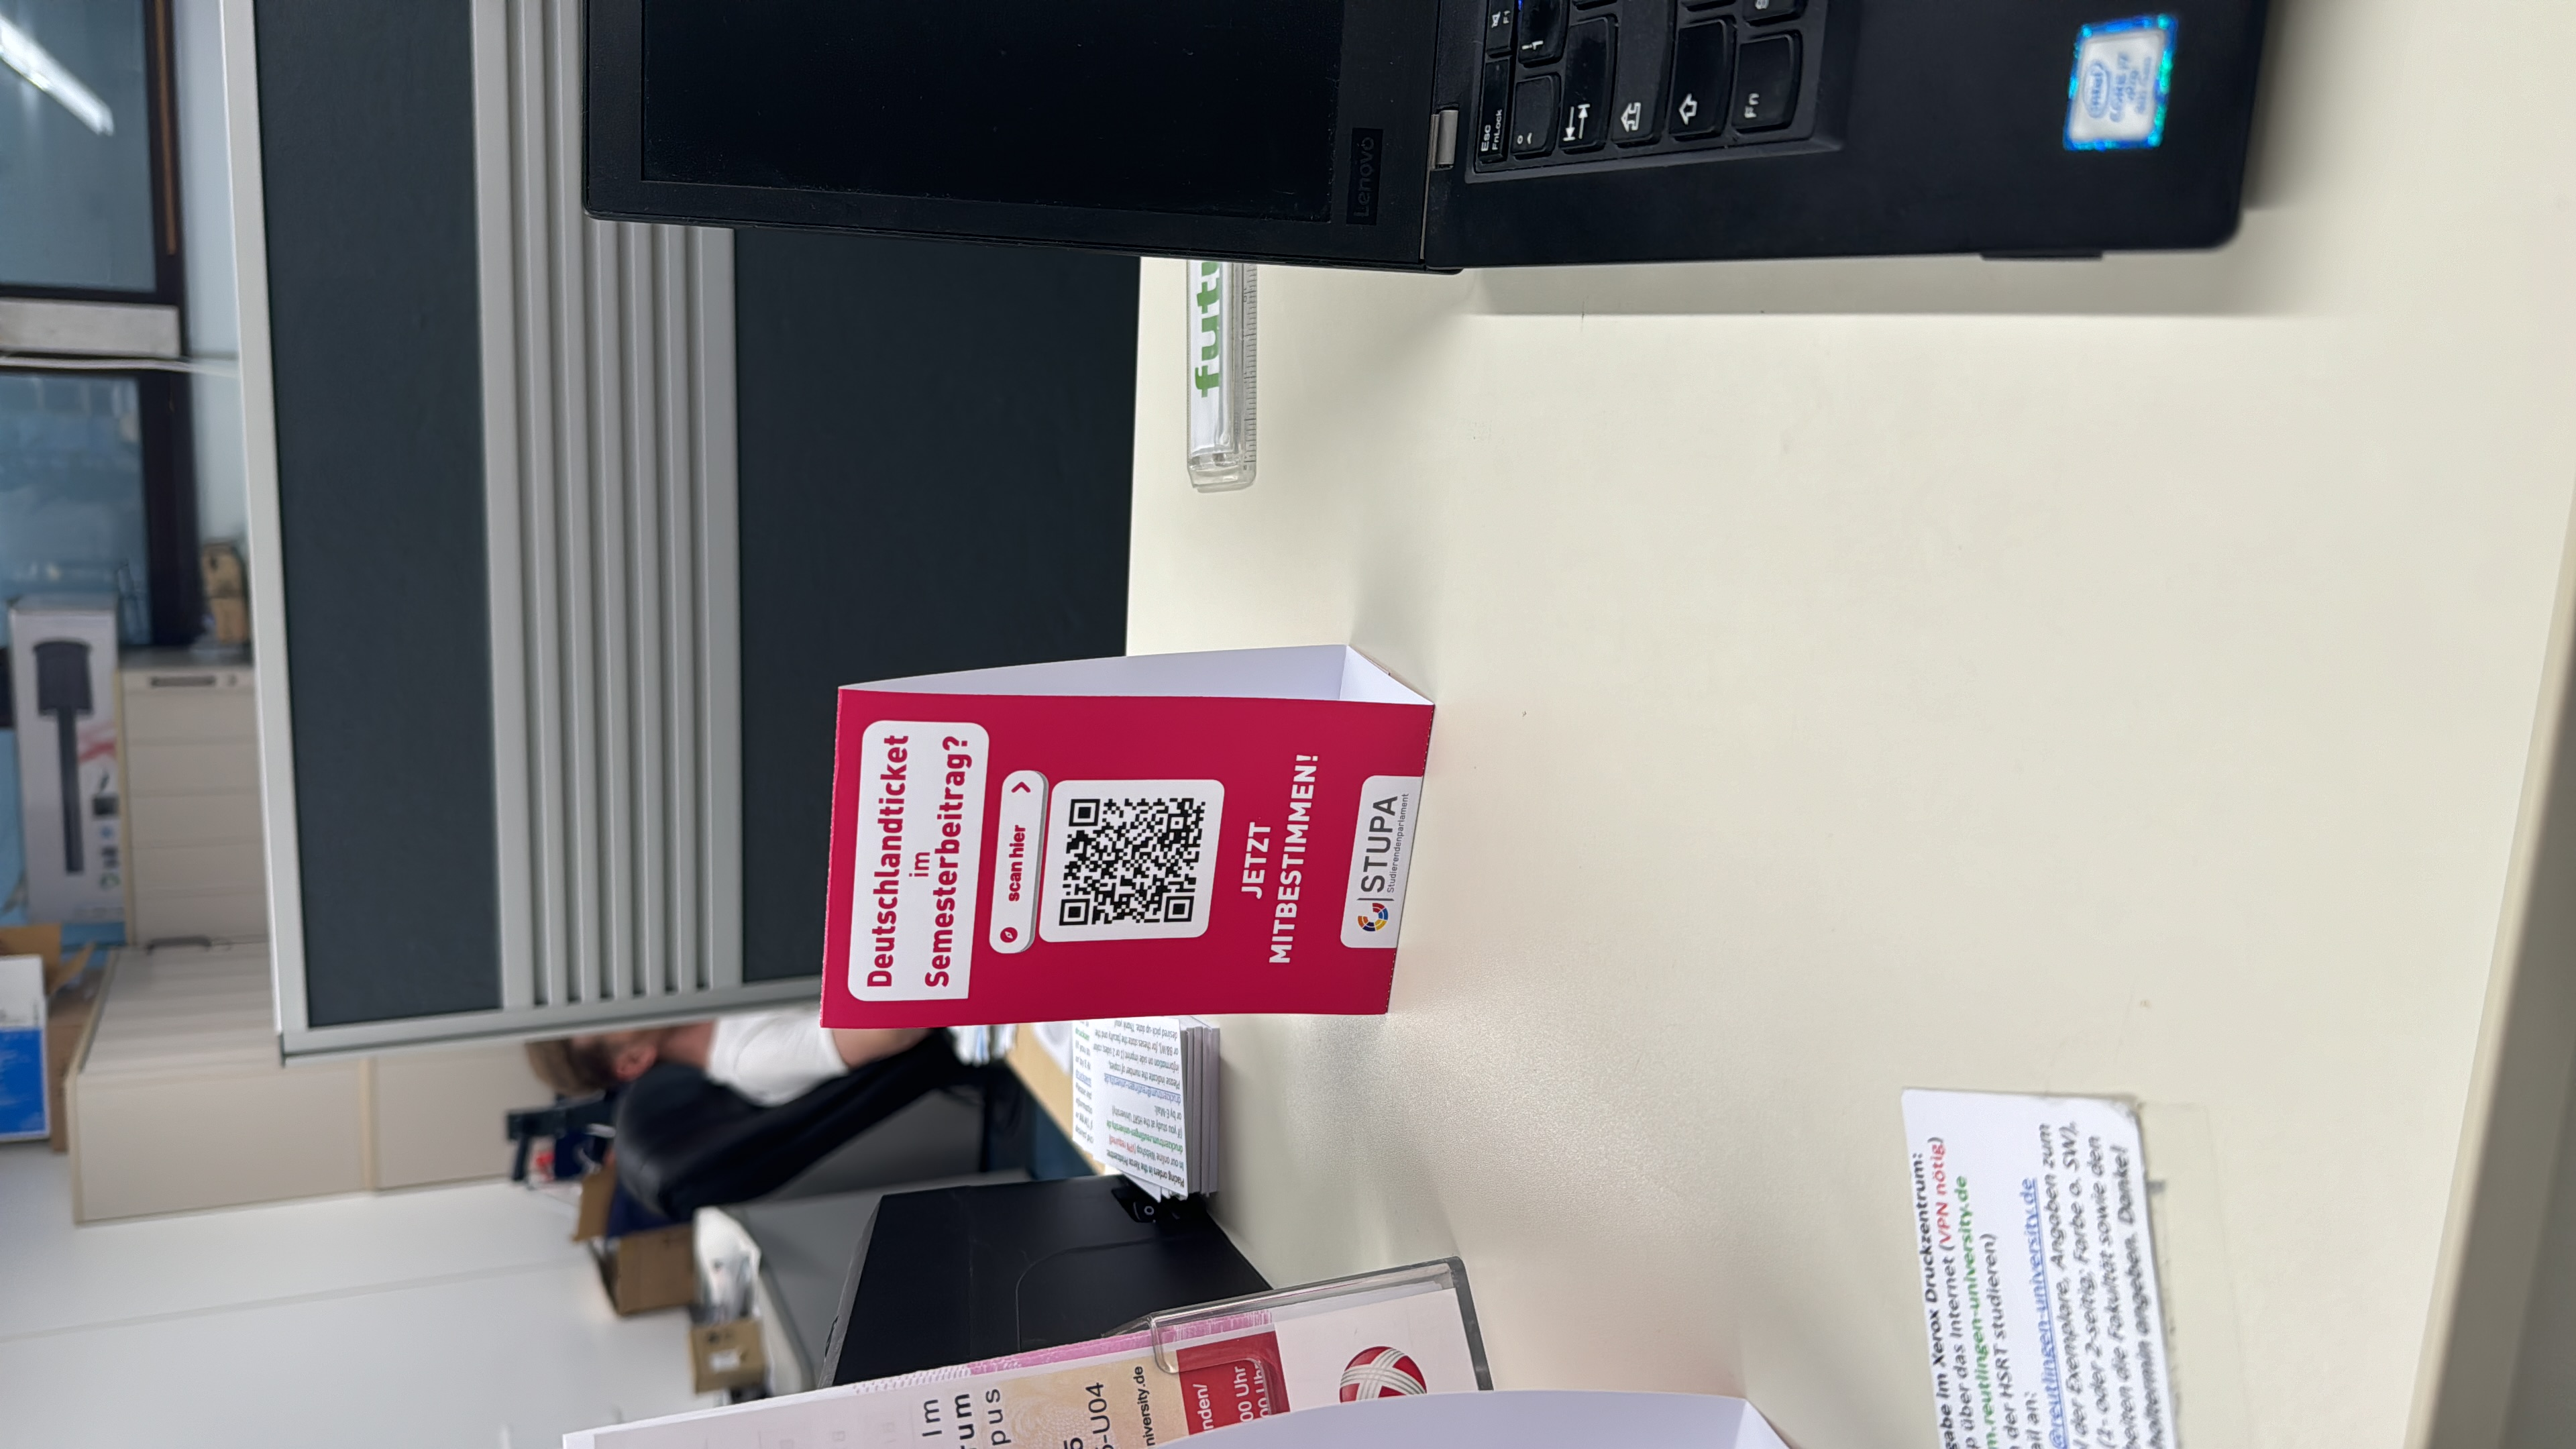
\includegraphics[width=0.8\textwidth, angle =-90]{Content/Images/tabletent.JPG}
        \caption{\gls{tt} 1}
        \label{fig:table-tent1}
    \end{figure}
    \columnbreak
    \begin{figure}[H]
        \vspace{0.3\textwidth}
        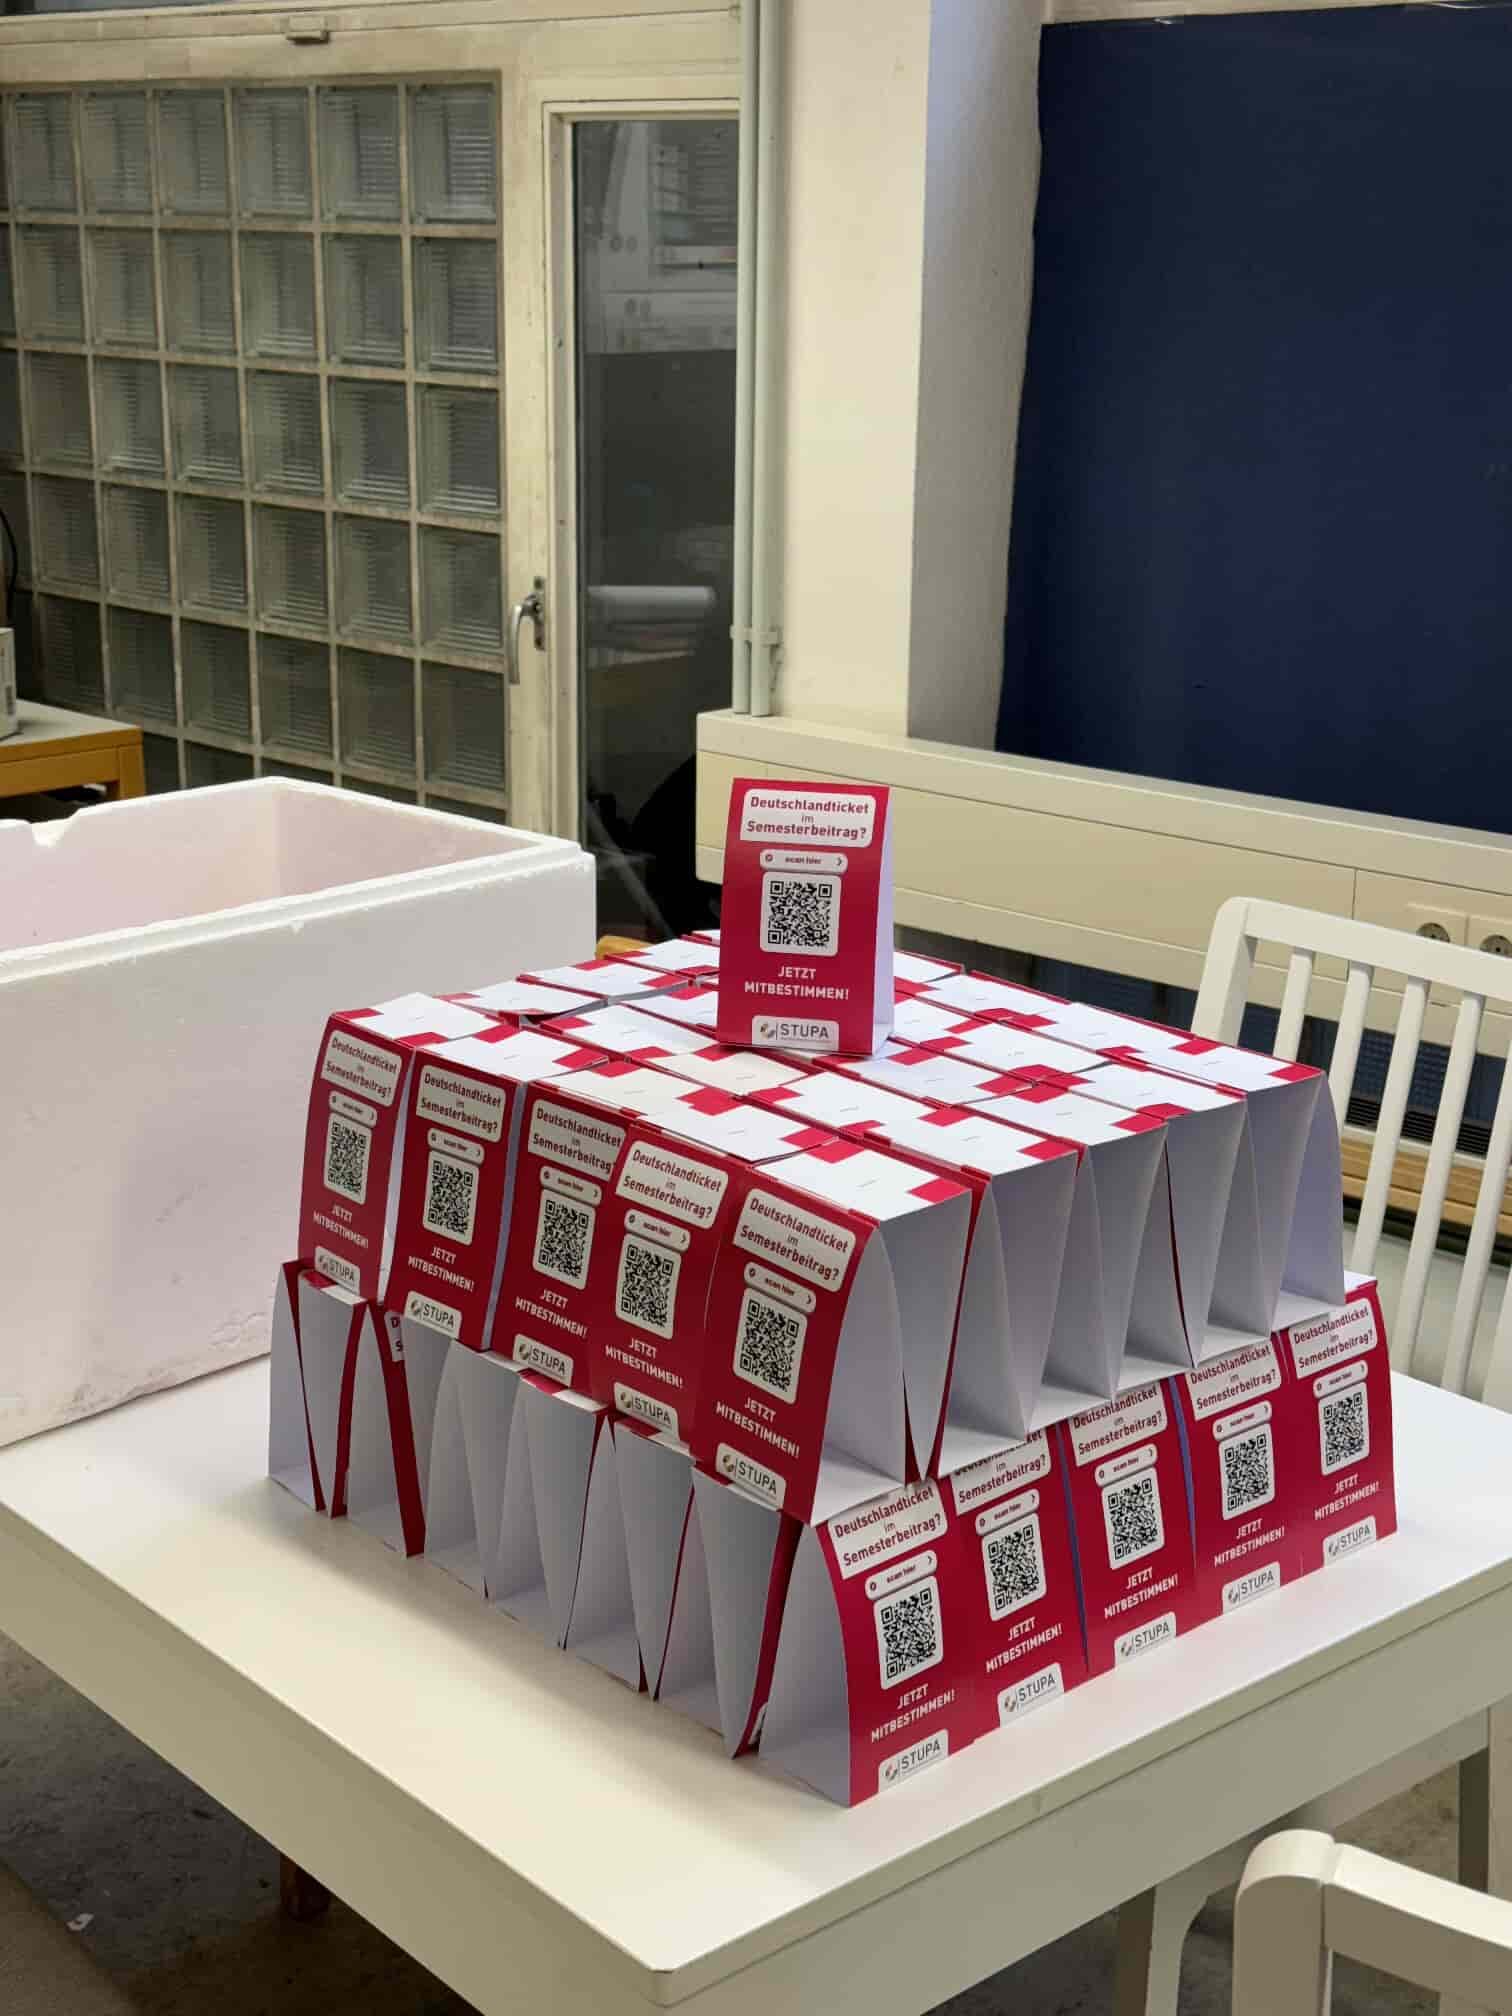
\includegraphics[width=0.8\textwidth]{Content/Images/tt_02.jpg}
        \caption{\gls{tt} 2}
        \label{fig:table-tent2}
    \end{figure}
    \columnbreak
    \begin{figure}[H]
        \vspace{0.3\textwidth}
        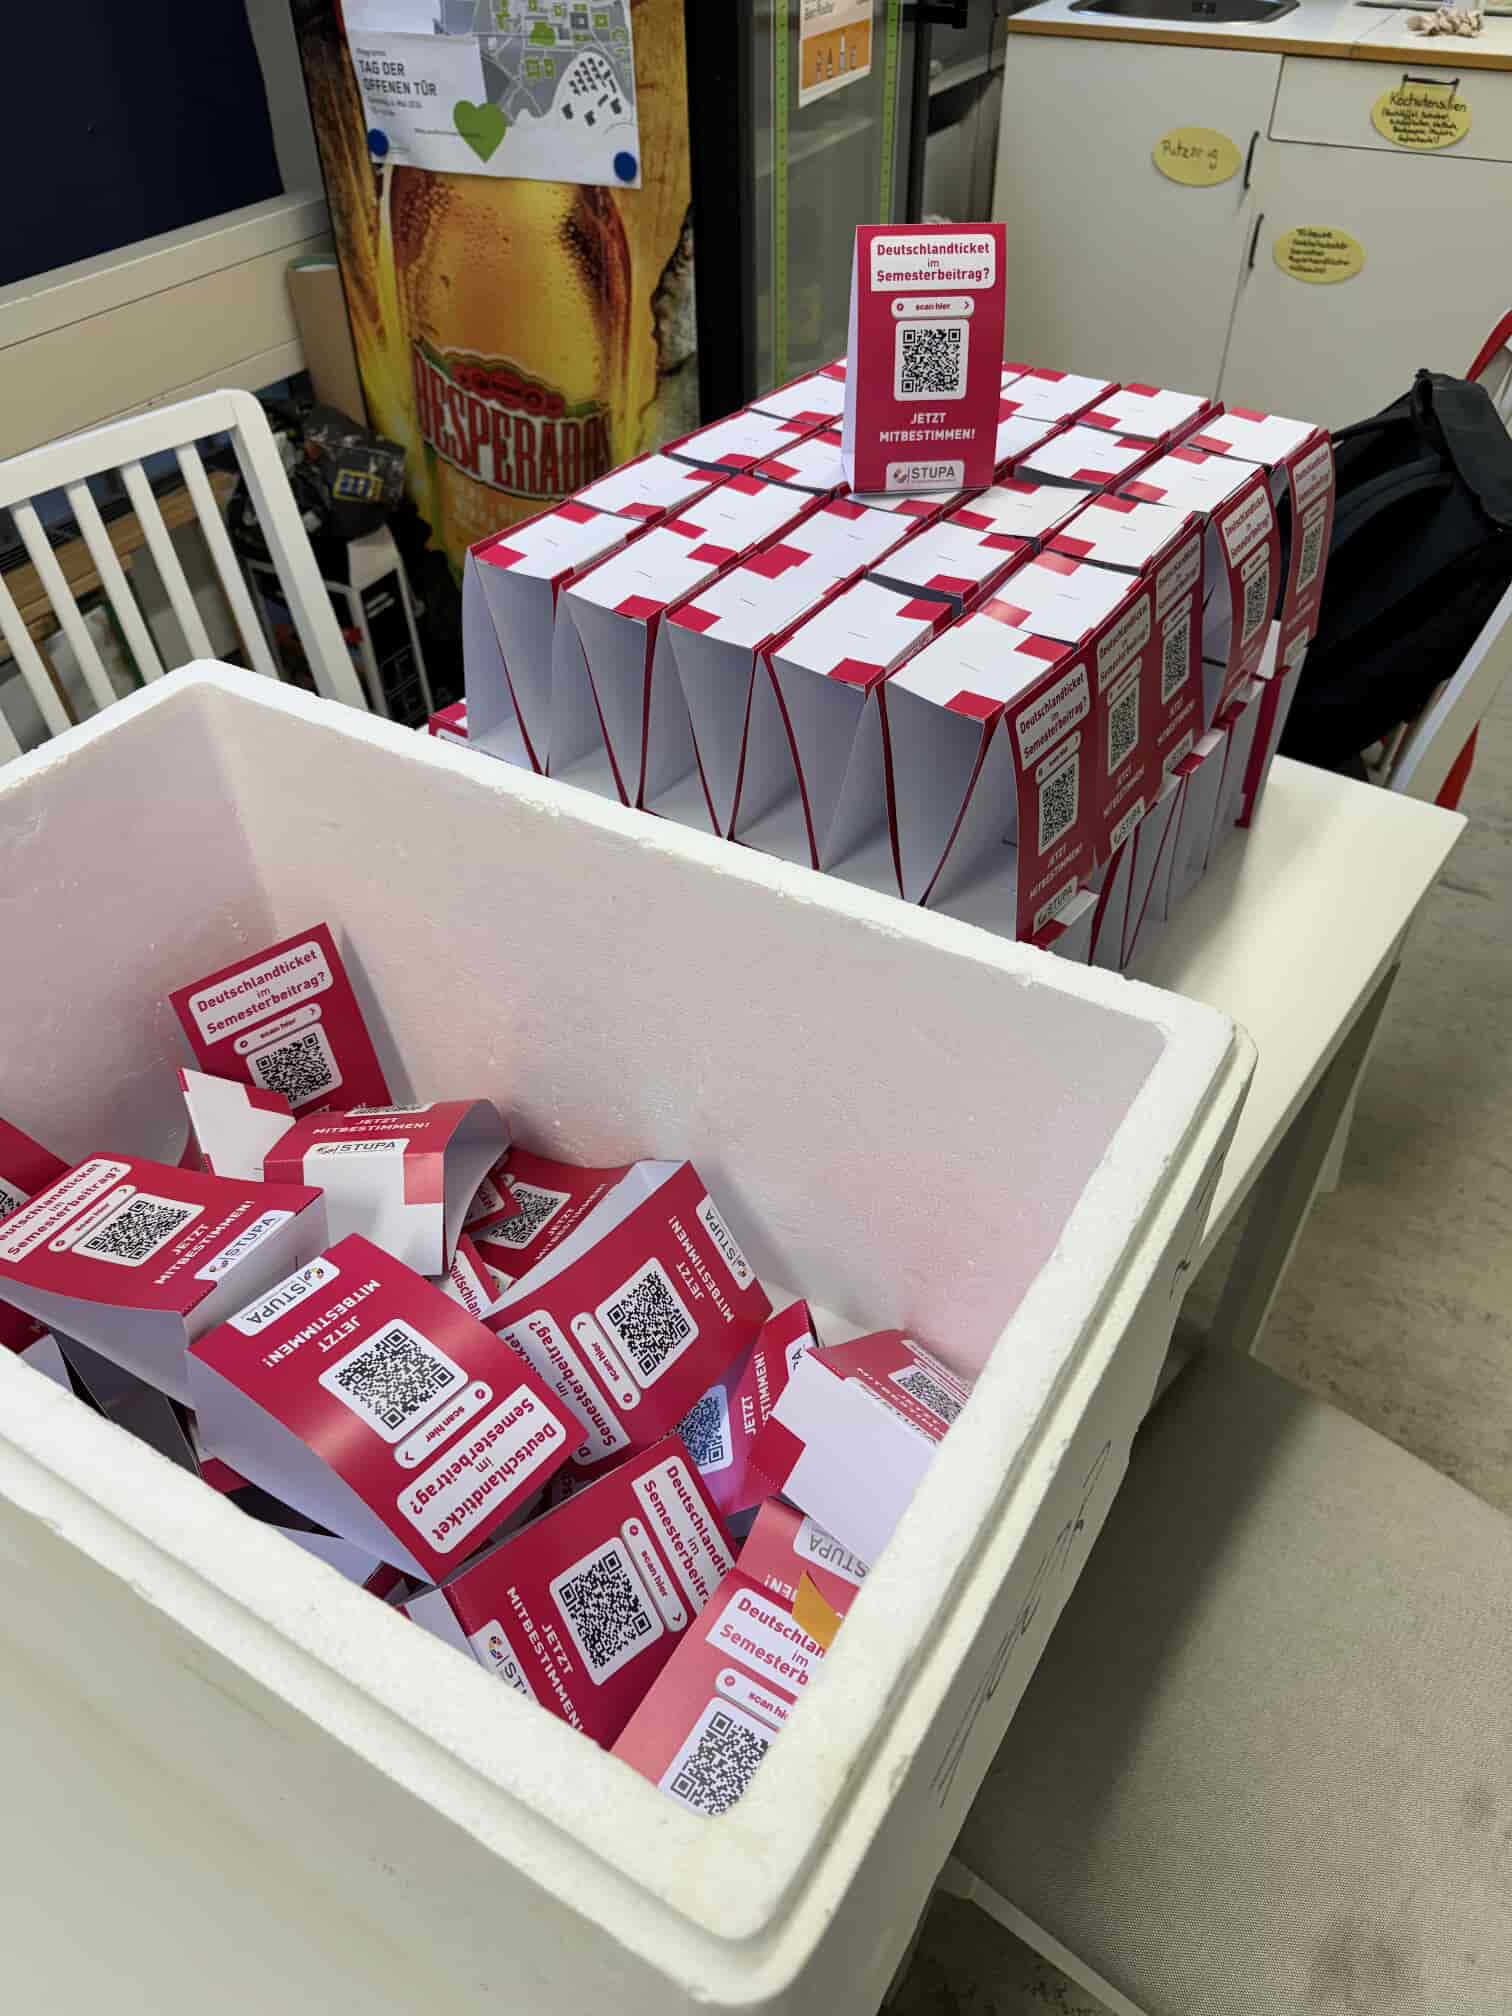
\includegraphics[width=0.8\textwidth]{Content/Images/tt_03.jpg}
        \caption{\gls{tt} 3}
        \label{fig:table-tent3}
    \end{figure}
\end{multicols}

\subsection{Survey Structure}

As shown below, the survey is divided into several parts. Most noticeable, information about the participant is collected to determine if they fall within our target group (students). Following this, the participant's level of knowledge is assessed. This question later confirmed our suspicion that many participants are not well-informed about the full solidarity model, reaffirming our choice to add a short informational text. Therefore ensuring that participants have a clear understanding of the model before they proceed with the survey. 

The participants were not allowed to go back to change an answer after they clicked next to ensure answers were not changed upon getting more information.

A keen observer would naturally notice that the sections are not listed in the order of their original IDs. As mentioned before the order of question groups was altered after initial testing. Since LimeSurvey did not allow us to easily change these ids they kept their original labels.

\textbf{The survey consists of the following sections:}

\begin{itemize}
    \item[\texttt{G01}] Participant Information:
    This section gathers demographic and contextual data to ensure the respondent is a student and to categorize responses based on relevant factors such as faculty and age.\\

    \item[\texttt{G02}] General Knowledge about the Deutschlandticket: Participants are asked to rate their knowledge about the Deutschlandticket and the full solidarity model to establish a baseline understanding before providing more detailed information.\\

    \item[\texttt{G04}] Current Means of Transportation: This section collects data on the current transportation habits of the participants, including the frequency and types of transport used, as well as related expenses and travel times.\\

    \item[\texttt{G05}] Importance of Climate Friendliness: Participants are asked about the importance they place on using environmentally friendly modes of transport, which helps contextualize their responses to subsequent questions about the Deutschlandticket.\\
    
    \item[\texttt{G03}] Stance on the Introduction of the Deutschlandticket: This section directly asks participants for their opinions on introducing the Deutschlandticket in the full solidarity model at Reutlingen University, capturing their initial reactions and support levels.\\

    \item[\texttt{G06}] Stance on Expected Conditions: Participants are queried about their views on the financial aspects of the proposed ticket model, including the fairness of a mandatory fee and whether the suggested monthly cost is reasonable.\\

    \item[\texttt{G07}] Expected Effect on Transport Use: This section explores how participants anticipate their use of public transport would change if the Deutschlandticket in the full solidarity model were introduced.\\

    \item[\texttt{G08}] Alternatives to the Proposed Model: An open-ended question allows participants to suggest other models or solutions, providing a space for feedback and additional ideas.\\
\end{itemize}

The structure ensures a logical flow from understanding participant demographics and current behaviors, through assessing knowledge and attitudes, to evaluating the potential impact and gathering alternative suggestions. This comprehensive approach aims to capture a holistic view of student opinions on the Deutschlandticket in the full solidarity model.
\subsection{Survey Tool: LimeSurvey}
LimeSurvey was chosen for its feature richness. It also has a good reputation as a tool for conducting scientific surveys. Additionally, we like that it is open source and can be self-hosted. LimeSurvey also allows for easy translation. We provided both an English and German Questionnaire.
\pagebreak
\chapter{Questionnaire}

\section{Final Questionnaire:}

\subsubsection{\texttt{G01} -- Questions about the participant}
\begin{displayquote}
    \texttt{G01Q01} -- \englishQuote{Which of the following categories applies to you?}\\
    \{Student | Employee | Professor/Lecturer | External(OTHER) \}\\\\
    \texttt{G01Q02} -- \englishQuote{Which faculty do you belong to? }\\
    \{INF | LS | ESB | TEC | TEX | OTHER\}\\\\
    \texttt{G01Q03} -- \englishQuote{Are you studying at Reutlingen University as part of an exchange program?}\\
    \{YES | NO\}\\\\
    \texttt{G01Q04} -- \englishQuote{Are you older than 26 years? }\\
    \{YES | NO\}\\\\
\end{displayquote}

\subsubsection{\texttt{G02} -- General knowledge about the Deutschlandticket in the full solidarity model}
\begin{displayquote}
    \texttt{G02Q01} -- \englishQuote{How would you rate your knowledge about the Deutschlandticket?}\\
    \{Very good | Rather good | Rather bad | Very bad\}\\\\
    \texttt{G02Q02} -- \englishQuote{How would you rate your knowledge about the full solidarity model at universities?}\\
    \{Very good | Rather good | Rather bad | Very bad\}\\\\
\end{displayquote}

\subsubsection{\texttt{G04} -- Current means of transportation}
\begin{displayquote}
    \texttt{G04Q01} -- \englishQuote{Which means of transport do you currently use the most to get to the university? [Ranking of three]}\\
    \{Bus and Train | Car | Bicycle | On Foot | Carpool\}\\\\
    \texttt{G04Q02} -- \englishQuote{How often do you currently use public transport to get to the university?}\\
    \{Daily | Several times a week | Less than once a week | Never\}\\\\
    \texttt{G04Q03} -- \englishQuote{How often do you otherwise use public transport?}\\
    \{Daily | Several times a week | Less than once a week | Never\}\\\\
    \texttt{G04Q04} -- \englishQuote{How much do you currently spend per month on your mobility? [Expenses in Euros]}\\
    \{Amount in Euros\}\\\\
    \texttt{G04Q05} -- \englishQuote{How far from the university do you live approximately? [Distance in Kilometers]}\\
    \{Distance in Kilometers\}\\\\
    \texttt{G04Q06} -- \englishQuote{How long does it usually take you to get to the university? [Duration in Minutes]}\\
    \{Duration in Minutes\}\\\\
    \texttt{G04Q07} -- \englishQuote{Do you currently have any of the following tickets?}\\
    \{Deutschlandticket | JugendBW-Ticket | Naldo-Semesterticket | Other\}\\\\
\end{displayquote}

\subsubsection{\texttt{G05} -- Importance of climate friendlyness to the participant}
\begin{displayquote}
    \texttt{G05Q01} -- \englishQuote{How important is the climate friendliness of the means of transport you use?}\\
    \{Very important | Rather important | Rather unimportant | Very unimportant\}\\\\
\end{displayquote}

\subsubsection{\texttt{G03} -- Stance on the introduction of the Deutschlandticket in the full solidarity model}\label{InfoText}

\begin{displayquote}
    
    \texttt{INFO TEXT} -- \englishQuote{What is the Deutschlandticket?}
    
    \englishQuote{The Deutschlandticket, also known as the 49-Euro ticket, is a monthly ticket for local public transport in Germany. For a price of 49 euro per month, it allows the use of all buses, trams, subways, S-Bahn and regional trains (2nd class) throughout Germany.
    Price: 49 euros per month. Validity: Nationwide on public transport, not on long-distance transport (ICE, IC, EC) and private long-distance buses. Aim: To facilitate the use of public transport, promote mobility and environmental friendliness. The ticket simplifies travel within Germany and offers a cost-effective and environmentally friendly alternative to private transport.
    What does full solidarity model mean?}

    \englishQuote{The full solidarity model enables students at Reutlingen University to obtain a public transport ticket valid throughout Germany for 29.40 Euro per month, which corresponds to 60\% of the regular ticket price of 49.00 Euro.
    Price: 29.40 Euro per month. Validity: Nationwide on all public transport (buses, trams, subways, S-Bahns, regional trains 2nd class). Solidarity principle: All students pay the same amount, regardless of frequency of use
    D-Ticket JugendBW: approx. 180 Euro per semester - of which 30Euro is a partial solidarity contribution in the semester fee - so the ticket price is approx. 150 Euro. Only valid up to 26 years of age. Recently equivalent to the Deutschlandticket.
    Naldo semester ticket: 141.90 Euro per semester, partial solidarity model. Only valid in the Naldo area!}\\   
\end{displayquote}

\begin{displayquote}
    \texttt{G03Q01} -- \englishQuote{What is your opinion on the introduction of the Deutschlandticket under the full solidarity model at Reutlingen University?}\\
    \{very Supportive | supportive | | opposed | strongly opposed\}\\\\
\end{displayquote}

\subsubsection{\texttt{G06} -- Stance on expected conditions}
\begin{displayquote}
    \texttt{G06Q01} -- \englishQuote{Do you consider the mentioned amount of 29.40Euro per month (180Euro per semester) to be reasonable?}\\
    \{YES | NO\}\\\\
    \texttt{G06Q02} -- \englishQuote{What amount do you think is appropriate?}\\
    \{Amount in Euros\}\\\\
    \texttt{G06Q03} -- \englishQuote{How fair do you find it that everyone pays the fee, even if they do not use the ticket?}\\
    \{Very fair | Rather fair | Rather unfair | Very unfair\}\\\\
\end{displayquote}

\subsubsection{\texttt{G07} -- Expected effect upon the participant}
\begin{displayquote}
    \texttt{G07Q01} -- \englishQuote{Do you expect that the Deutschlandticket in the full solidarity model would change your use of public transport?}\\
    \{Significantly | Somewhat | Not at all\}\\\\
\end{displayquote}

\subsubsection{\texttt{G08} -- Alternatives to the proposed model}
\begin{displayquote}
    \texttt{G08Q01} -- \englishQuote{What alternatives to the Deutschlandticket in the full solidarity model would you suggest?}\\
    \{ Free Text \}
\end{displayquote}

\pagebreak

%\pagecolor{lightgrey}
\section{UI Elements:}
This section gives an exemplary visual overview of our Questionnaire. Pictograms and arrows illustrate the possible actions.\\
\vspace{20pt}

\begin{comment}
\begin{multicols}{2}
    {
        \begin{figure}[H]
            \centering
            \fbox{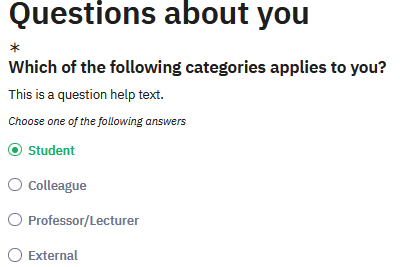
\includegraphics[width=.95\textwidth]{Content/Images/sureyouhaveachoice.png}}
            \caption{\texttt{G01Q01}}
            \label{fig:enter-label}
        \end{figure}
        \begin{figure}[H]
            \centering
            \fbox{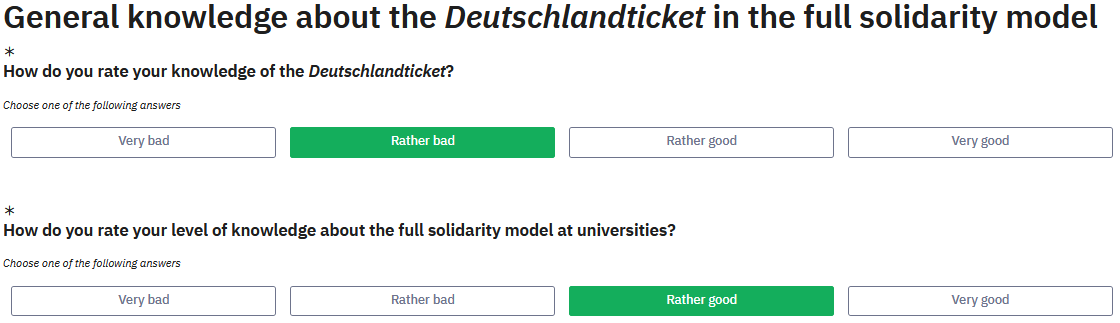
\includegraphics[width=.95\textwidth]{Content/Images/range.png}}
            \caption{\texttt{G02Q01-02}}
            \label{fig:enter-label}
        \end{figure}
        \begin{figure}[H]
            \centering
            \fbox{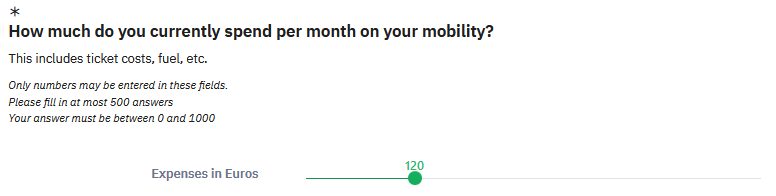
\includegraphics[width=.95\textwidth]{Content/Images/slider.png}}
            \caption{\texttt{G04Q04}}
            \label{fig:enter-label}
        \end{figure}
        
    } \columnbreak {
        \begin{figure}[H]
            \centering
            \fbox{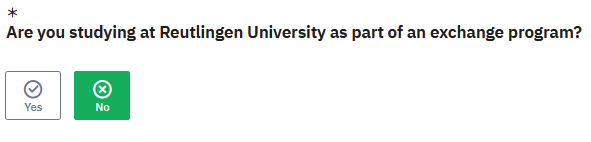
\includegraphics[width=.95\textwidth]{Content/Images/yesOrNo.png}}
            \caption{\texttt{G01Q03}}
            \label{fig:enter-label}
        \end{figure}
        \begin{figure}[H]
            \centering
            \fbox{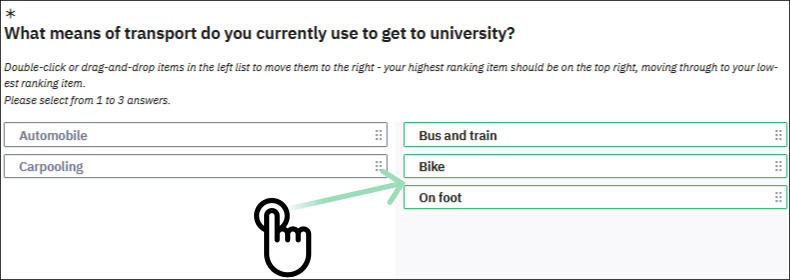
\includegraphics[width=.95\textwidth]{Content/Images/ranking.png}}
            \caption{\texttt{G04Q01}}
            \label{fig:G04Q01RankingQuestionScreenshot}
        \end{figure}
        \begin{figure}[H]
            \centering
            \fbox{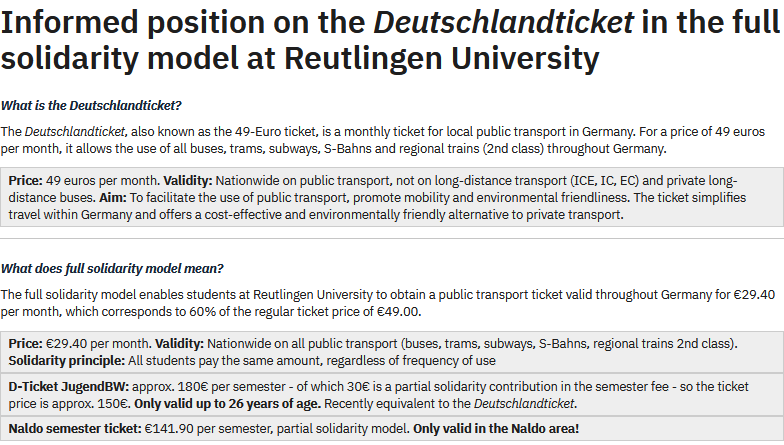
\includegraphics[width=.95\textwidth]{Content/Images/infotext.png}}
            \caption{\texttt{G03}}
            \label{fig:enter-label}
        \end{figure}
    }
\end{multicols}
\begin{multicols}{1}
    {
        \begin{figure}[H]
            \centering
            \fbox{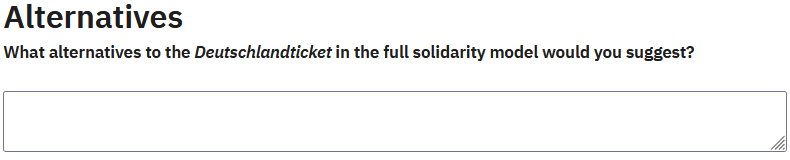
\includegraphics[width=.95\textwidth]{Content/Images/freetext.png}}
            \caption{\texttt{G08Q01}}
            \label{fig:enter-label}
        \end{figure}
    }
\end{multicols}
\end{comment}
\chapter{Results}



\section{Code}
The Graphs where created using Python with the data-analysis-framework \textbf{\texttt{pandas}} and \textbf{\texttt{matplotlib.pyplot}} for the graphs. The complete code can be found on the attached \href{https://github.com/frederikbeimgraben/Statistik-und-Biometrie-Praesentation}{git repository}.


\section{Participation and Representativeness}
\subsection{Participation}
\input{Build/TeX/ParticipationText.tex}

\begin{multicols}{2}
    {
        \input{Build/TeX/Figures/OptimumFacultyDistribution.tex}
    } \columnbreak {
        \input{Build/TeX/Figures/FacultyDistribution.tex}
    }
\end{multicols}

Through targeted marketing, we successfully achieved a balanced distribution of respondents, as seen in \ref{fig:FacultyDistribution}.  
The  data, provided by the StuPa, is current as of March 2024. The faculty distributions are as follows: \textbf{ESB 41.4\%, INF 20.6\%, TEC 17.0\%, TEX 11.4\%, LS 9.6\%} - visualised in Figure \ref{fig:OptimumFacultyDistribution}.

\subsection{Representativeness}
\begin{multicols}{1}
    \input{Build/TeX/Figures/FacultyDifference.tex}
    \columnbreak
    {
        As seen in \ref{fig:FacultyDifference}, the faculty distribution of the survey participants approximately mirrors the actual distribution at Reutlingen University.
        The deviation at the ESB-Faculty is likely due to a large portion of international students, who might not have been reached by our marketing efforts. At the time of writing this (11.7.24), we had not yet received a response from the university administration regarding the current number of international students at the ESB Faculty, so we cannot verify this assumption.
        Furthermore for some students the semester had already ended while the survey was still running.
    }
\end{multicols}

\pagebreak
\section{Findings}
\subsection{Answer to the Research Question: Level of acceptance among the students of Reutlingen University for a \gls{dt} in the full solidarity model?}
\begin{center}
    \englishQuote{What is the level of acceptance among the students of Reutlingen University for a \gls{dt} in the full solidarity model?}
\end{center}

To determine the support of the \gls{dt} in general we used the following questions:

\begin{enumerate}
    \item[\texttt{G03Q01}] \englishQuote{What is your opinion on the introduction of the Deutschlandticket under the full solidarity model at Reutlingen University?}
    \item[\texttt{G06Q01}] \englishQuote{Do you think the stated amount of 29.40 Euro per month (180 Euro per semester) is reasonable?}
\end{enumerate}
Both questions are asked after the participants have been informed about the \gls{dt} and the full solidarity model. The information text can be found in \ref{InfoText}. Additionally the time spent on the \ref*{InfoText} was measured and participants with less than 15 seconds were excluded from the analysis.\\\\
Not adjusted for the group representations the overall results are visualized in \ref{fig:SupportDTFSM} and \ref{fig:AmountReasonable}:\\
\ref{fig:SupportDTFSM} llustrates a strong interest in the \gls{dt}. Notably, 48.8\% of respondents are very supportive, 32.8\% are supportive, while only 8.2\% are opposed, and 10.3\% are very opposed.

\ref{fig:SupportDTFSM} demonstrates a significant interest in the \gls{dt}. Specifically, 48.8\% of respondents are \englishQuote{very supportive}, 32.8\% are \englishQuote{supportive}, while only 8.2\% are \englishQuote{opposed} and 10.3\% are \englishQuote{very opposed}. This indicates that there is strong overall support for the concept of the Deutschlandticket.

This indicates that while there is strong overall support for the concept of the \gls{dt}, the current pricing structure may be a significant barrier to broader acceptance.

\begin{multicols}{2}
    {
        \input{Build/TeX/Figures/SupportDTFSM.tex}
    } \columnbreak {
        \input{Build/TeX/Figures/AmountReasonable.tex}
    }
\end{multicols}

\clearpage

\begin{enumerate}
    \item[\texttt{G06Q02}] \englishQuote{What amount do you think is appropriate? }
\end{enumerate}

\begin{multicols}{2}
    \input{Build/TeX/Figures/AmountsConsideredReasonable.tex}
    \columnbreak
    \input{Build/TeX/AmountsConsideredReasonable.tex}
\end{multicols}

Additionally we asked the participants whether they perceived the fact that all students would have to pay the same amount as fair with:

\begin{enumerate}
    \item[\texttt{G06Q01}] \englishQuote{How fair do you find it that everyone pays the fee, even if they do not use the ticket?}
\end{enumerate}

\begin{multicols}{2}
    \input{Build/TeX/Figures/Fairness.tex}
    \columnbreak
    \input{Build/TeX/Fairness.tex}
\end{multicols}

\pagebreak
\subsection{Modes of Transportation by Faculty}

\begin{comment}
\begin{figure}[H]
    \centering
    \includesvg[width=0.7\textwidth]{Content/auswertungen_svgs/faculty_vs_transportation_rank_1.svg}
    \caption{\texttt{G01Q02:G04Q01} Distance vs. Mode of Transportation}
    \label{fig:modesByFaculty}
\end{figure}
\end{comment}



\begin{enumerate}
    \item[\texttt{G04Q01}] \englishQuote{What means of transport do you currently use to get to university? }
\end{enumerate}
Question G04Q01 is a ranking question, where participants were asked to rank their top 3 modes of transportation to the university. The data was then grouped by faculty to identify any differences in transportation habits across faculties. The results are visualized in \ref{fig:modesByFaculty}.
Overall, the data shows that public transportation and cars are the predominant modes of transport among students. Public transportation is widely used, reflecting its accessibility and convenience. Bicycles are also popular, indicating a trend towards eco-friendly and cost-effective travel.
 Car usage varies significantly across faculties, suggesting differences in the need for flexibility and convenience. It would also be interesting to have more specific information on the home location of the students as suggested in \ref{FutureConsiderations}.
 
%So man muss bei ranking eben anders analysieren... erklaerung dazu HIER  dann die grafen und dann was das bedeutet dann kann man es noch mit 

\subsection{Primary Mode of Transportation vs. Distance}
\begin{comment}
\begin{figure}[H]
    \centering
    \includesvg[width=0.7\textwidth]{Content/auswertungen_svgs/distance_vs_transportation.svg}
    \caption{\texttt{G04Q01:G04Q05} Distance vs. Mode of Transportation}
    \label{fig:distanceVsTransportation}
\end{figure}
\end{comment}
\ref{fig:distanceVsTransportation} shows that car usage increases with distance. Furthermore this graph also shows that even in the range of $(0;10]$ km car usage still makes up roughly 40\%. According to Sabine Merkens, our mobility officer, this matches earlier findings from the mobility survey. 
Interestingly, we can see an early peak in car usage between 20-30 km, which can be attributed to the proximity to the city center and the convenience of commuting within this range. This is followed by a noticeable dent between 30-40 km, which can be explained by the presence of the two nearby big cities, Stuttgart and Tübingen, and their well-developed infrastructure. These cities likely offer robust public transportation options and amenities that reduce the necessity of car usage. Consequently, residents and commuters might prefer using public transport over driving, leading to the observed reduction in car usage in this specific distance rang

However, it is important to note that these are mere speculations, as we currently lack concrete data to substantiate these claims. Therefore, in the "Future Considerations" \ref{FutureConsiderations} section, it is recommended that future surveys include a form of location data from respondents. This addition would provide more precise insights and help validate the observed patterns in car usage.

This graph was created by dividing the data in to bins of 10 kilometers on the \texttt{G04Q05} column. We dropped the interval from 50 to 100 km due to too few data points.

\subsection{Distance vs. Time per Mode of Transportation}
\begin{comment}
\begin{figure}[H]
    \centering
    \includesvg[width=0.7\textwidth]{Content/auswertungen_svgs/time_vs_distance_scatter.svg}
    \caption{\texttt{G04Q05:G04Q06} Distance vs. Time}
    \label{fig:distanceVsTime}
\end{figure}
\end{comment}
In \ref{fig:distanceVsTime} we can see the relation between distance to the campus and time needed to reach campus for each primary mode of mobility. The x-axis is scaled logarithmically to increase readablity. From the graph we can deduct that those that use public transportation to reach campus need significantly more time for the same distance when compared to those that use a car.

\subsection{Primary Mode of Transportation vs. Money spent}
\begin{comment}
\begin{figure}[H]
    \centering
    \includesvg[width=0.7\textwidth]{Content/auswertungen_svgs/transportation_vs_money.svg}
    \caption{\texttt{G04Q04:G04Q01} Transportation vs. Money}
    \label{fig:modeVsMoney}
\end{figure}
\end{comment}
The boxplot shown in Figure \ref{fig:modeVsMoney} represents the relationship between different modes of transportation (x-axis) and their respective costs in euros (y-axis). Each box corresponds to a specific mode of transportation and depicts the distribution of costs associated with that mode.

\begin{itemize}
    \item \textbf{Median Cost:}
    \begin{itemize}
        \item The median cost (black line) varies significantly across different modes of transportation.
        \item \textbf{Car:} The median cost is around 200 euros.
        \item \textbf{By foot:} The median cost is around 100 euros.
        \item \textbf{Public transportation:} The median cost is slightly above 50 euros.
        \item \textbf{Bicycle:} The median cost is around 25 euros.
        \item \textbf{Carpooled:} The median cost is around 200 euros.
    \end{itemize}

    \item \textbf{Spread of Costs:}
    \begin{itemize}
        \item \textbf{Car:} The costs are relatively concentrated with a range from around 100 to 250 euros, indicating a higher cost but less variation.
        \item \textbf{By foot:} The costs have a wider range, with a large interquartile range indicating more variability in money spent.
        \item \textbf{Public transportation:} The costs are the lowest and show a tight range, suggesting consistent and lower spending.
        \item \textbf{Bicycle:} Similar to public transportation, bicycle costs are low and show minimal variability.
        \item \textbf{Carpooled:} The costs have a very wide range, with some extreme values indicating a high variability in spending.
    \end{itemize}

    \item \textbf{Outliers:}
    \begin{itemize}
        \item There are outliers in the categories \textbf{By foot} and \textbf{Carpooled}, indicating that some individuals spend significantly more than others within these groups.
    \end{itemize}

    \item \textbf{General Insights:}
    \begin{itemize}
        \item \textbf{Cars and Carpooling} tend to have higher median costs compared to other modes of transportation, with carpooling showing a wider spread and more variability in costs.
        \item \textbf{Public transportation and bicycles} are the most cost-effective options, with low and consistent spending.
        \item \textbf{Walking} has varied costs, indicating that participants who walk to the university still incur expenses for other forms of transportation, likely using cars or carpools for travel beyond university commuting. This suggests that public transportation does not entirely eliminate the need for a car for many participants."

    \end{itemize}

    \item \textbf{Cost Efficiency:}
    \begin{itemize}
        \item For individuals looking for cost-efficient transportation, public transportation and bicycles seem to be the best options.
        \item Carpooling, while having a wide range of costs, might still be more cost-efficient than driving a car alone.
    \end{itemize}
\end{itemize}

\chapter{Future Considerations and Lessons Learned}
\label{FutureConsiderations}
Below are some additional ideas and potential improvements. 
\begin{enumerate}
    \item \englishQuote{How close is a participant living to a relevant public transportation node (e.g. train stations) }
    \item \englishQuote{Coordinates of participants home (drop pin on map)}
    \item \englishQuote{How much time is spent on each question $\rightarrow$ to check engagement with info-text}
    \item \englishQuote{Dynamic links for ad campaigns enable the measurement of campaign performance (e.g., approximately 15\% on Instagram). However, differentiation between email, posters, and tablets is currently not possible. It is also feasible to segment the results by buildings to identify where ads are most effective. The optimal scenario would involve using specific QR codes for each poster and logging the position of each poster.}
    
\end{enumerate}